%\documentclass{article}
\documentclass[journal,12pt,twocolumn]{IEEEtran}

% Language setting
% Replace `english' with e.g. `spanish' to change the document language
\usepackage[english]{babel}

% Set page size and margins
% Replace `letterpaper' with `a4paper' for UK/EU standard size
%%\usepackage[letterpaper,top=2cm,bottom=2cm,left=3cm,right=3cm,marginparwidth=1.75cm]{geometry}

% Useful packages
\usepackage[utf8]{inputenc}
\usepackage{enumitem}
\usepackage{multicol}
\usepackage{ragged2e}
\usepackage{amsmath}
\usepackage{amssymb}
\usepackage{graphicx}
\let\vec\mathbf
\newcommand{\myvec}[1]{\ensuremath{\begin{pmatrix}#1\end{pmatrix}}}
\usepackage{array}
\usepackage{blindtext}
%\usepackage[paperwidth=10cm]{geometry}
\usepackage{tkz-euclide}
%\usepackage{tikz}
\usetikzlibrary{
  circuits.logic,
  circuits.logic.US,
  positioning
}
\usepackage[colorlinks=true, allcolors=blue]{hyperref}

\title{Optimization Assignment}
\author{Navya Valmeekam}
\begin{document}
\providecommand{\norm}[1]{\left\lVert#1\right\rVert}
\maketitle
\begin{tableofcontents}
\section{Problem}
\noindent A dealer wishes to purchase a number of fans and sewing machines. He has only Rs. 5,760 to invest and has a space for at most 20 items. A fan costs him Rs.360 and a sewing machine Rs.240. His expectation is that he can sell a fan at a profit of Rs. 22 and a sewing machine at a profit of Rs. 18. Assuming that he can sell all the items that he can buy, how should he invest his money in order to maximize the profit? Formulate this as a linear programming problem and solve it graphically. 
\\
\\
\\
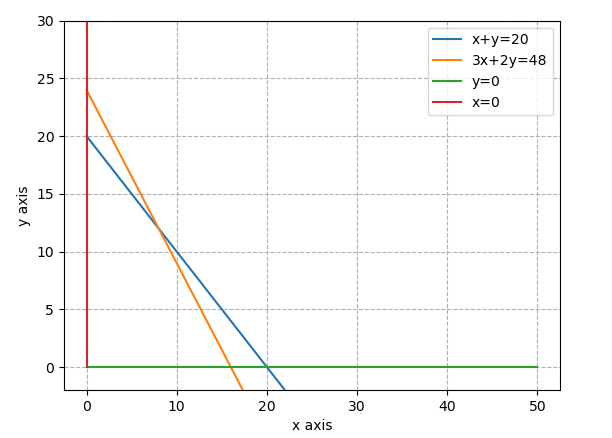
\includegraphics[scale=0.43]{graph.png} 
%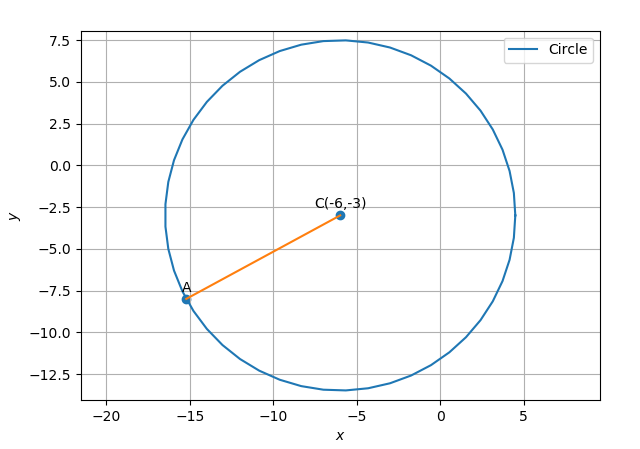
\includegraphics[scale=0.4]{circle.png} 
\begin{center}
Graph
\end{center}
\vspace{0.3cm}
\section{Solution}
Let number of fans be x and number of sewing machines be y\\
According to given problem, problem can be formulated as,\\
\vspace{2cm}
\begin{equation}
	P=\vec{max}(22\vec{x}+18\vec{y})
\end{equation}
Where P is the maximum profit\\
Constraints can be formulated based on given data
Given Dealer can buy at most 20 items\\
\begin{equation}
	\vec{x}+\vec{y}\leq20
\end{equation}
Dealer can invest Rs.5,760
\begin{equation}
	360\vec{x}+240\vec{y}\leq5760
\end{equation}
this can be simplified as,\\
\begin{equation}
	3\vec{x}+2\vec{y}\leq48
\end{equation}
x,y must be non-negative
\begin{equation}
	\vec{x}\geq0
\end{equation}
\begin{equation}
	\vec{y}\geq0
\end{equation}
Equations (2) and (4),(5) and (6) can be expressed in vector forms as\\
\begin{equation}
\begin{pmatrix}
1 & 1\\
3 & 2\\
-1 & 0\\
0 & -1\\
\end{pmatrix}
	\vec{x}\\
\leq\\
\begin{pmatrix}
20\\
48\\
0\\
0
\end{pmatrix}
\end{equation}
Equation (1) can also be expressed in vector form as\\
\begin{equation}
	P=\vec{max}(22 \hspace{0.1cm} 18)
	\begin{pmatrix}
		\vec{x}\\
		\vec{y}
	\end{pmatrix}	
\end{equation}
Solving above equations using cvxpy, we get\\
\begin{equation}
	\vec{P_{max}}=392
\end{equation}
\begin{equation}
	\vec{x}=
\begin{pmatrix}
8\\
12\end{pmatrix}
\end{equation}
\end{tableofcontents}
\end{document}
